% Create a Table of Contents in Beamer
\documentclass[10pt,t]{beamer}
% Theme choice:
\usetheme{Singapore}
\useoutertheme{sidebar}
\usecolortheme{seahorse}
\setbeamercolor{titlelike}{bg=white}
\setbeamercolor{frametitle}{bg=white}
%\setbeamertemplate{frametitle}[default][left]
\setbeamertemplate{navigation symbols}{}

\usepackage{graphicx}
\usepackage{amsmath}
\usepackage{amsfonts}
\usepackage{amssymb}
\usepackage{amsthm}
\usepackage{ulem}
\usepackage{listings}

% Title page details: 
\title{Chapter 1c: Prediction in Linear Regression} 
\author{Taylor Okonek \& Charlie Wolock}
\date{\today}


\begin{document}
	% Title page frame
	\begin{frame}
	\titlepage 
\end{frame}

\begin{frame}{Learning objectives}
By the end of Chapter 1c, you should be able to:
\begin{itemize}
	\item Understand and explain the difference between the scientific goals of prediction vs. inference
	\item Be able to compute fitted values in \texttt{R} and by hand
	\item Understand the importance of training vs. testing data, and how to create training and testing datasets in \texttt{R}
	\item Determine the predictive accuracy of a linear regression analysis using $R^2$
	\item Compute the Mean Squared Error for a regression model
	\item Understand and explain the bias-variance tradeoff
\end{itemize}
\end{frame}

% Outline frame
\begin{frame}{Outline}
\tableofcontents
\end{frame}

\AtBeginSection[ ]
{
\begin{frame}{Outline}
\tableofcontents[currentsection]
\end{frame}
}

% Presentation structure
% Prediction vs. Inference - difference in goals
% Fitted values review & examples - in R and by hand
% Training and testing data
% Measures of prediction accuracy
% - R^2
% - MSE
% Bias-variance tradeoff


\section{Prediction vs. Inference}

\begin{frame}{Prediction vs. Inference}
So far in this course, our goal has been to estimate the association between a predictor of interest and our outcome.

\vspace{0.3cm}

In Chapter 1b, we discussed the potential need to adjust for additional variables in our regression model (confounders, precision variables, effect modifiers). The inclusion of additional variables was motivated by scientific questions about \textit{association}, which led us to conduct \textit{statistical inference}.

\vspace{0.3cm}

When our scientific question involves \textit{prediction}, we have a different goal in mind: develop an algorithm based on current data that, when we plug in future data, predicts the outcome well.
\end{frame}

\begin{frame}{Prediction vs. Inference}
In loose terms:
\vspace{0.3cm}

\textcolor{blue}{Prediction:} using a model to predict outcomes for new data points

\vspace{0.3cm}

\textcolor{blue}{Inference:} understanding the relationships between variables (typically a predictor of interest and an outcome)
\end{frame}

\begin{frame}{Inference: scientific questions}
With inference, we are able to answer questions such as\dots

\vspace{0.3cm}

\begin{itemize}
	\item Are individuals with a specific genetic variable more susceptible to certain diseases later in life?
	\item Is there an association between access to antenatal clinics and maternal mortality in rural areas?
	\item Was a certain public health intervention associated with improved health outcomes for a community?
	\item Is a new vaccine effective at reducing the risk of getting a disease, or perhaps a severe case of the disease?
\end{itemize}

\end{frame}

\begin{frame}{Prediction: scientific questions}
With prediction, we are instead interest in questions such as\dots

\vspace{0.3cm}

\begin{itemize}
	\item How do predict risk of type II diabetes based on an individual's medical history?
	\item Can we accurately classify tumors in the central nervous system?
	\item What is the under-5 mortality rate at the state level for a country where we have no reliable census or vital registration data?
	\item Based on the videos a person has watched on YouTube, can we give them accurate suggestions for videos they would like to watch next?
\end{itemize}

\vspace{0.3cm} \pause

* questions like the last one are asked by companies all the time, including YouTube, TikTok, Netflix, or any company that provides some form of media or involves targeted advertising 
\end{frame}


\section{Fitted values}

\begin{frame}{Fitted values}
How do we actually use a model to \textit{predict} something? We use fitted values!

\vspace{0.3cm}

From Chapter 1a:

\vspace{0.3cm}

\textcolor{blue}{Fitted value}: the value of the response predicted from your regression \pause

\vspace{0.3cm}

Consider the linear regression model
$$
E[Y \mid X_1, \dots, X_p] = \beta_0 + \beta_1 X_1 + \dots + \beta_p X_p
$$

If we fit this model, we obtain coefficient estimates $\hat{\beta}_0, \dots \hat{\beta}_p$, and we can plug them into our regression equation to get fitted values $\hat{Y}$:
$$
\hat{Y} = \hat{\beta}_0 + \hat{\beta}_1 X_1 + \dots + \hat{\beta}_p X_p
$$

\end{frame}

\begin{frame}{Fitted values}
Each observation in our dataset gets a fitted value, based on their covariates values $X_1, \dots, X_p$. If we denote each observation by $i = 1, \dots, n$ for $n$ total observations, we can write these fitted values as
$$
\hat{Y}_i = \hat{\beta}_0 + \hat{\beta}_1 X_{i, 1} + \dots + \hat{\beta}_p X_{i, p}
$$

In two dimensions, fitted values are not too difficult to visualize (as we will do on the next slide). In higher dimensions (i.e., when we have more than one covariate in our model), fitted values are less easy to visualize.

\vspace{0.3cm}

Fitted values \textit{are} the predicted values (predictions) for each observation in our dataset!

\end{frame}

\begin{frame}{Fitted values: Visualizing in two dimensions}
In two dimensions (where we have only one predictor $X_1$), we can visualize fitted values on a scatter plot:
\vspace{0.3cm}

\centering 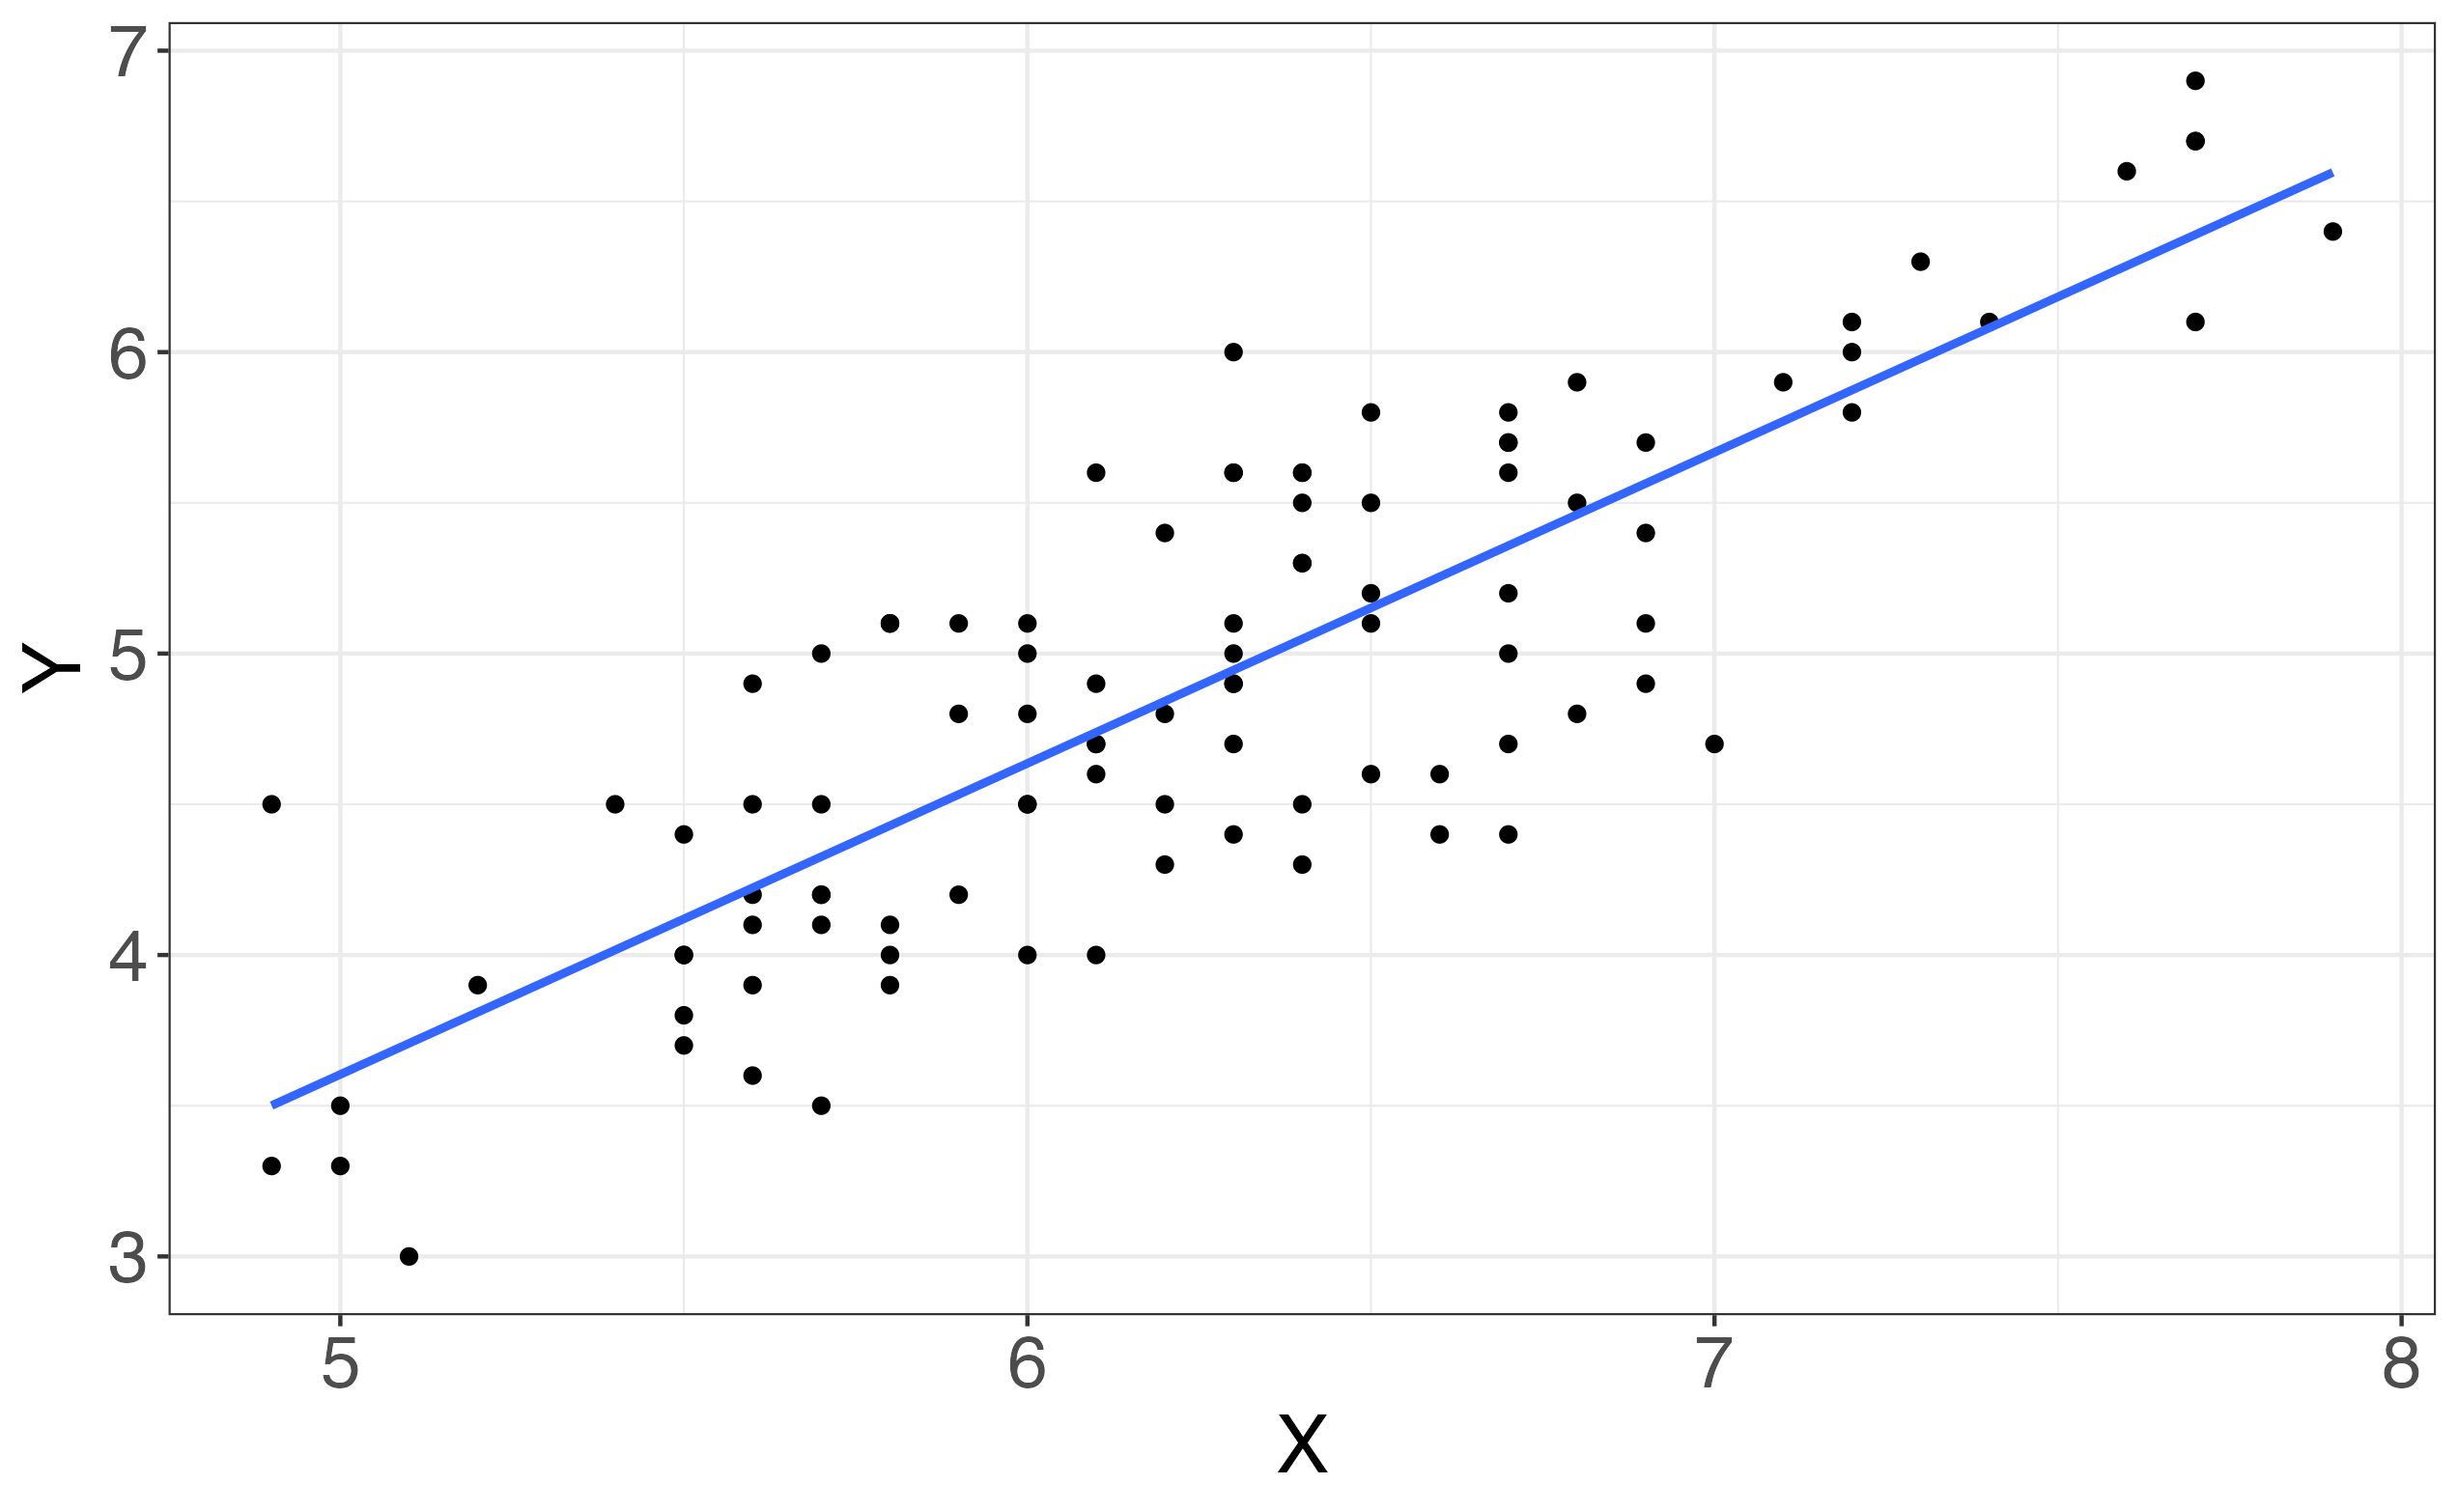
\includegraphics[scale=0.4]{fitted_vals1.png}
\end{frame}

\begin{frame}{Fitted values: Visualizing in two dimensions}
In two dimensions (where we have only one predictor $X_1$), we can visualize fitted values on a scatter plot:
\vspace{0.3cm}

\centering 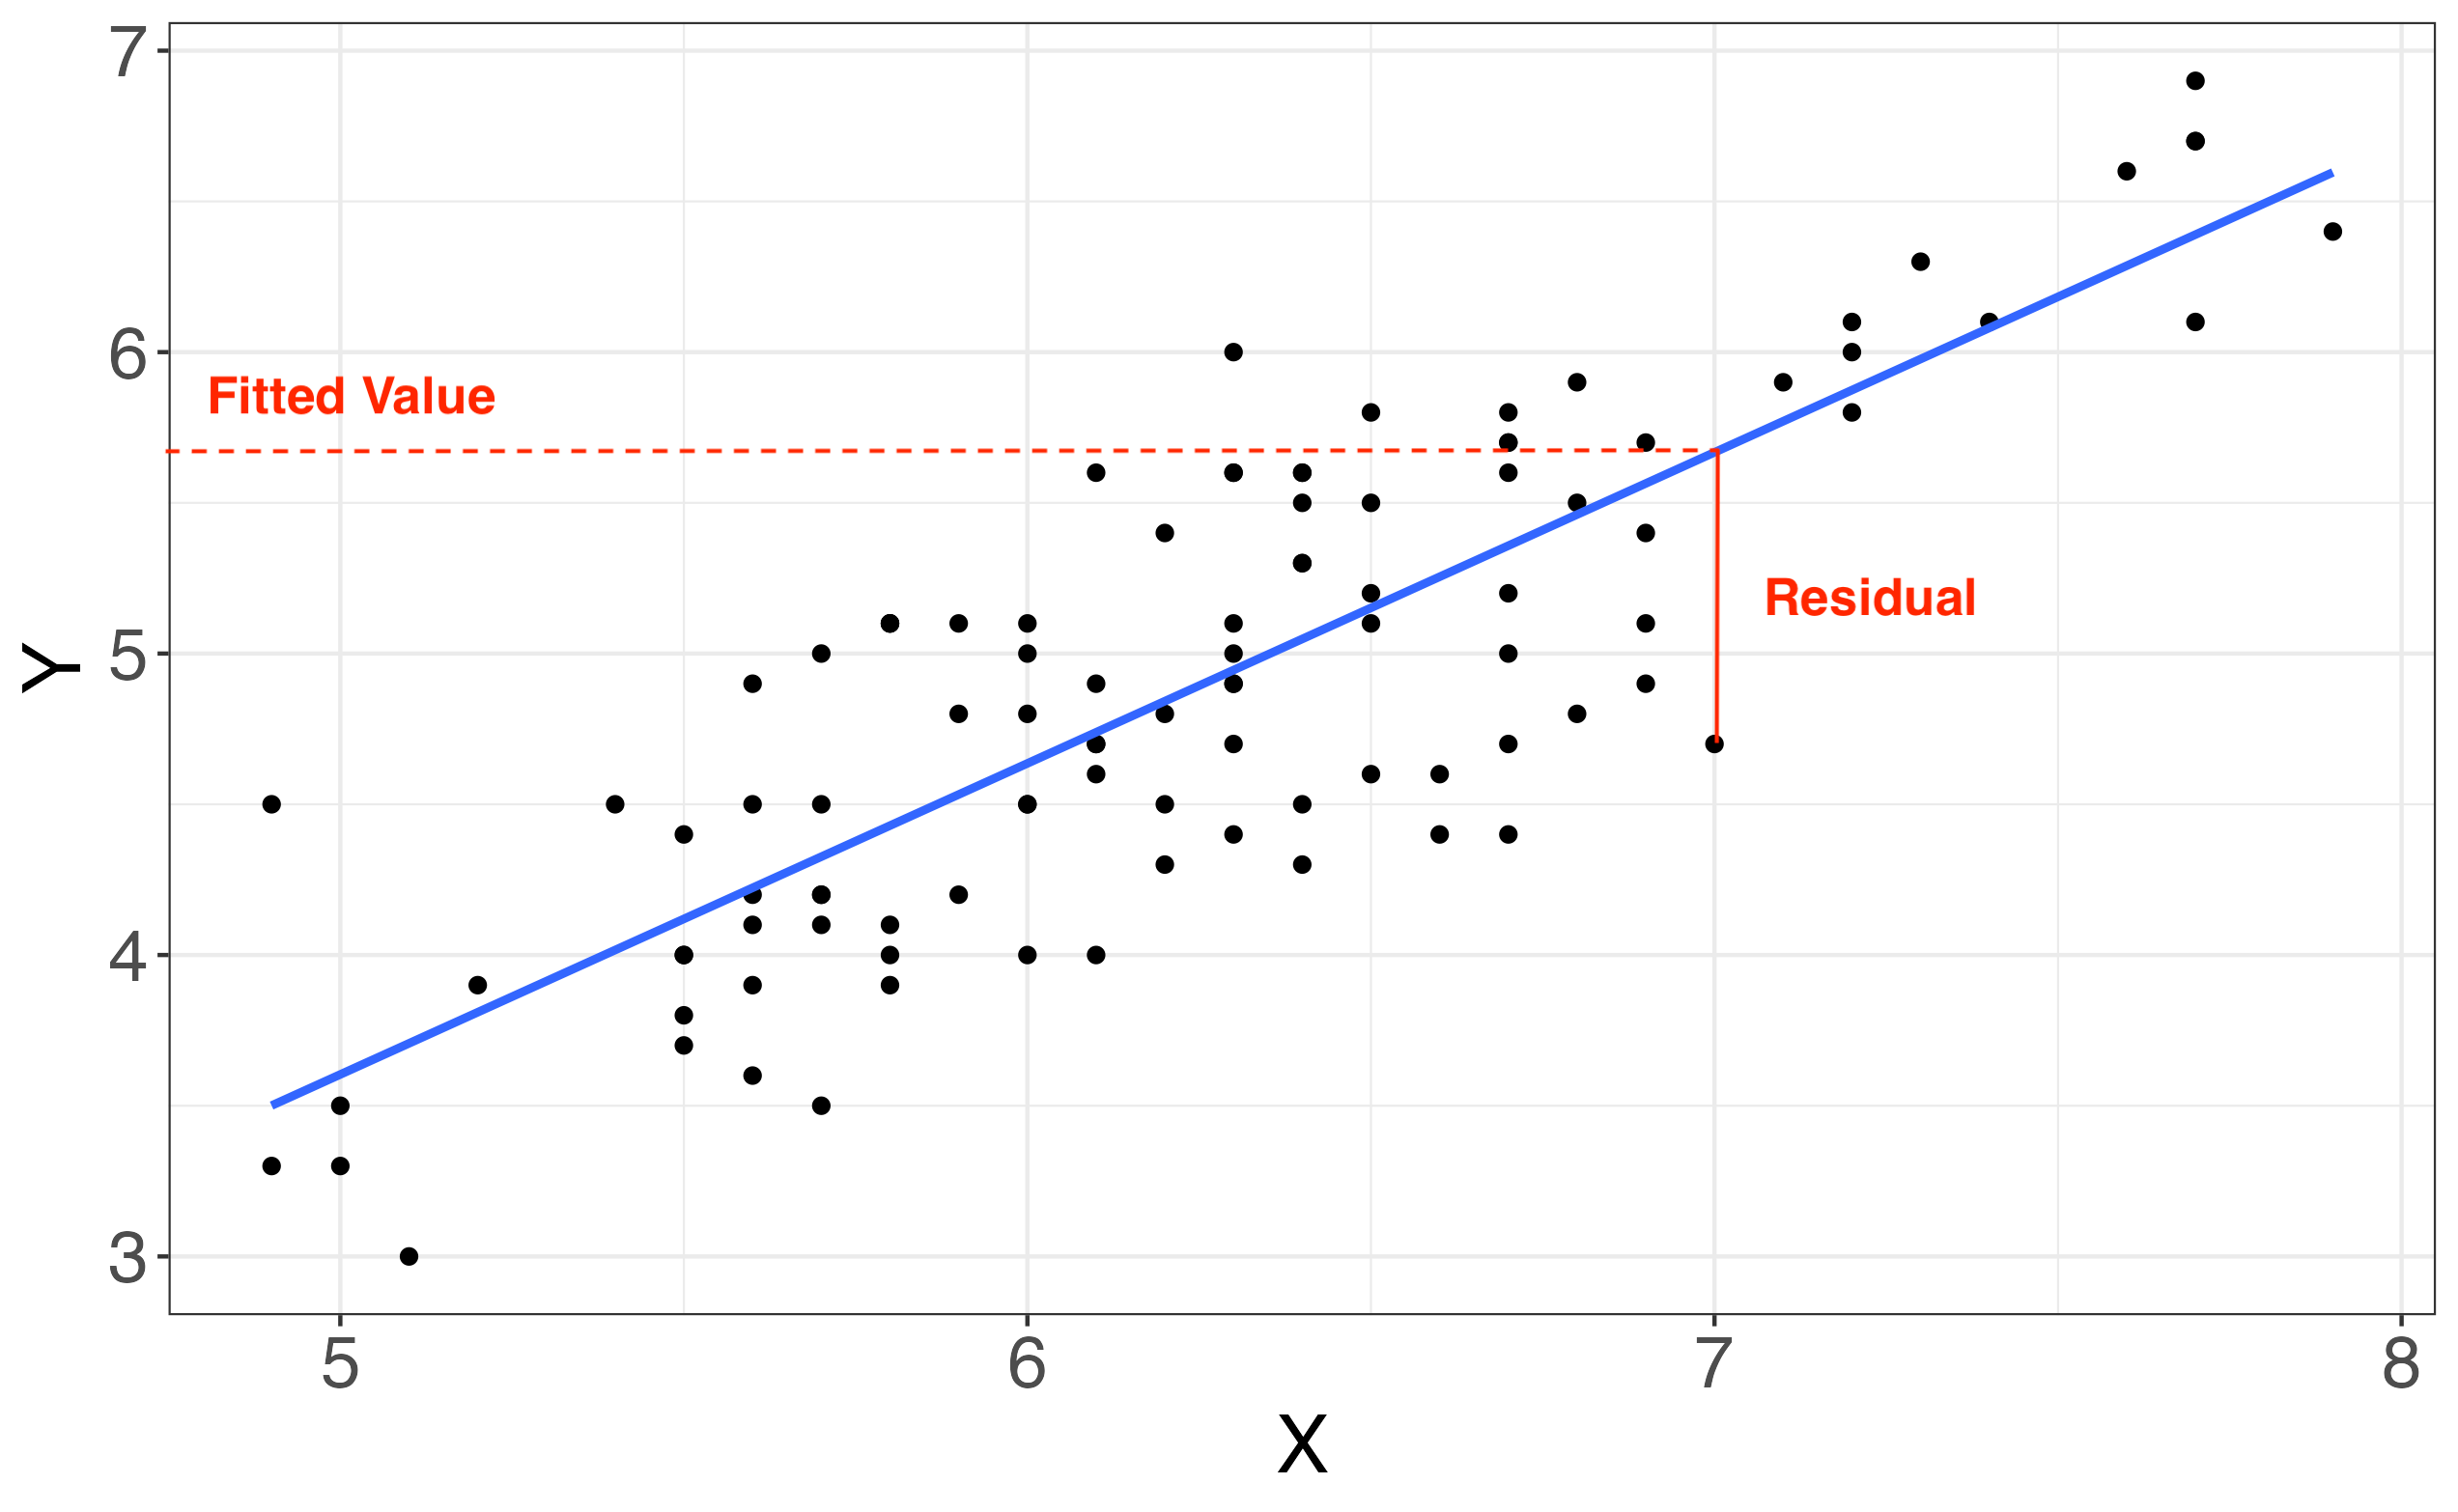
\includegraphics[scale=0.4]{fitted_vals2.png}
\end{frame}

\begin{frame}{Fitted values and prediction}
Fitted values allow us to obtain predictions for each observation in our dataset. Suppose we suddenly get covariate data ($X_1, \dots, X_p$) for a new observation, but we do not know their outcome $Y$. 

\vspace{0.3cm} 

\textcolor{blue}{Question:} Without re-fitting our linear regression model, how can we obtain a prediction for this observation based on their covariates? \pause

\vspace{0.3cm}

We can plug their covariates into our regression equation! If our dataset already has $n$ observations, we can denote this new observation as the $(n + 1)$'th observation, and write
$$
\hat{Y}_{n + 1} = \hat{\beta}_0 + \hat{\beta}_1 X_{(n + 1), 1} + \dots + \hat{\beta}_p X_{(n + 1), p}
$$

We can calculate by $\hat{Y}_{n + 1}$ by hand or in \texttt{R}, and we'll see examples of both.

\end{frame}

\begin{frame}{Prediction: Example in \texttt{R}}

Suppose we want are interested in predicting a baby's birthweight based on birth parent's age, marital status, whether or not they smoke during pregnancy, and weight prior to pregnancy. We can fit the appropriate regression model in \texttt{R}:

\vspace{0.2cm}

\centering 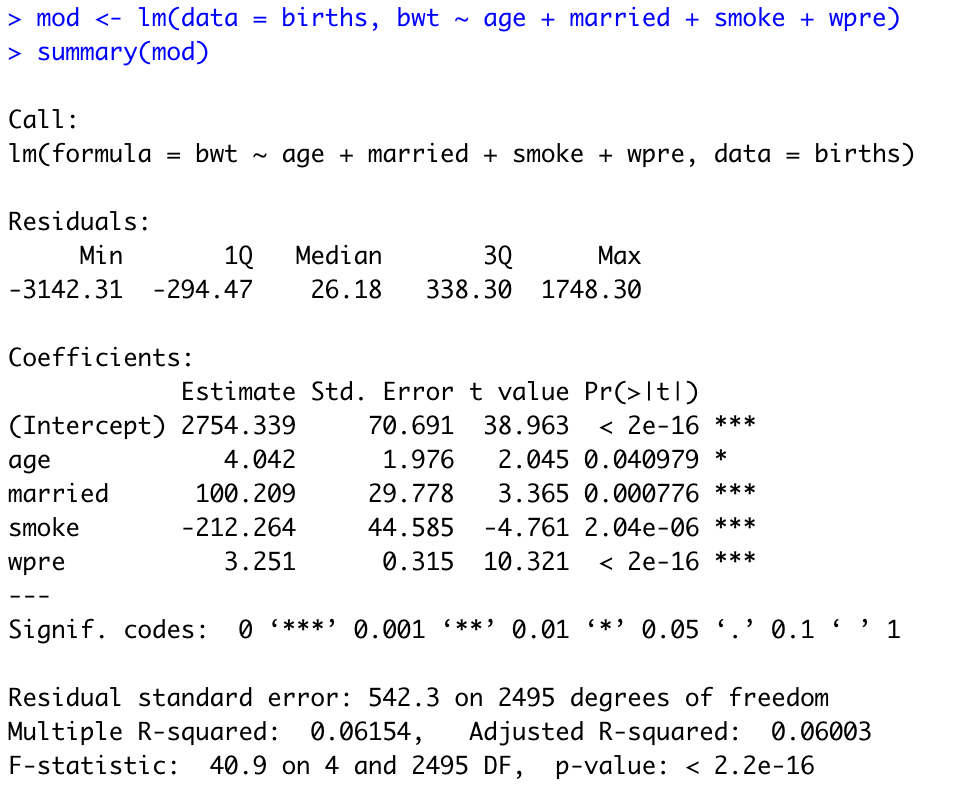
\includegraphics[scale=0.35]{predict_reg.png}
\end{frame}

\begin{frame}{Prediction: Example in \texttt{R}}
Extracting the coefficient estimates from this model and plugging them into our regression equation, we get
\begin{align*}
\hat{Y} = & 2754.339 + 4.042 \times \text{age} + 100.209 \times \text{married} \\
& - 212.264 \times \text{smoke} + 3.251 \times \text{wpre} 
\end{align*} \pause

What is our best estimate of a baby's birthweight born to a birth parent who is 25 years old, married, does not smoke, and weighed 150 pounds prior to pregnancy? \pause

\begin{align*}
\hat{Y} = & 2754.339 + 4.042 \times 25 + 100.209 \times 1 \\
& - 212.264 \times 0 + 3.251 \times 150  \\
& = 3443.223 \text{ grams}
\end{align*}

\end{frame}

\begin{frame}{Prediction: Example in \texttt{R}}
Extracting the coefficient estimates from this model and plugging them into our regression equation, we get
\begin{align*}
\hat{Y} = & 2754.339 + 4.042 \times \text{age} + 100.209 \times \text{married} \\
& - 212.264 \times \text{smoke} + 3.251 \times \text{wpre}
\end{align*}

What is our best estimate of a baby's birthweight born to a birth parent who is 15 years old, unmarried, smokes, and weighed 120 pounds prior to pregnancy? \pause

\begin{align*}
\hat{Y} = & 2754.339 + 4.042 \times 15 + 100.209 \times 0 \\
& - 212.264 \times 1 + 3.251 \times 120  \\
& = 2992.807 \text{ grams}
\end{align*}

\end{frame}

\begin{frame}{Prediction: Example in \texttt{R}}
Extracting the coefficient estimates from this model and plugging them into our regression equation, we get
\begin{align*}
\hat{Y} = & 2754.339 + 4.042 \times \text{age} + 100.209 \times \text{married} \\
& - 212.264 \times \text{smoke} + 3.251 \times \text{wpre}
\end{align*}

What is our best estimate of a baby's birthweight born to a birth parent who is 80 years old, married, does not smoke, and weighed 1000 pounds prior to pregnancy? \pause

\begin{align*}
\hat{Y} = & 2754.339 + 4.042 \times 80 + 100.209 \times 1 \\
& - 212.264 \times 0 + 3.251 \times 1000  \\
& = 6428.78 \text{ grams}
\end{align*}

* 6428.78 grams is approximately 13.3 pounds

\end{frame}

\begin{frame}{Prediction: extrapolation}
Our birthweight estimate for a birth parent who is 80 years old, married, does not smoke, and weighed 1000 pounds prior to pregnancy was 13.3 pounds. 13.3 pounds is not unheard of for a baby, but is very large.

\vspace{0.3cm}

\textcolor{blue}{Question:} Within our dataset, the oldest observed individual was 46 years old, and the individual with the highest pre-pregnancy birthweight was 350 pounds. Is it reasonable to make a prediction for an individual with covariate values so far outside of our dataframe? \pause

\vspace{0.3cm}

\textcolor{blue}{Answer:} It depends! If we believe that the observed linear relationship holds for covariate values even outside of those observed in our dataframe, then we may be okay. However, we have no way of knowing from our data whether or not the linear relationship holds for covariate values outside of our dataframe, because we don't observe them! 

\vspace{0.3cm}

\small Predicting values outside of the range of our observed data is known as \textcolor{blue}{extrapolation}, and is unreasonable to do in many scientific settings.

\end{frame}

\begin{frame}{Prediction: Example in \texttt{R}}
Rather than calculate predictions by hand, it is often useful to do this in \texttt{R}, and we can make predictions for more than one observation at a time. As in Chapter 1a to obtain fitted values for our observed data, we can use the \texttt{predict} function to get fitted values for new data as well.

\vspace{0.3cm}

To get fitted values for our observed data, we just call the \texttt{predict} function on our modeling object \texttt{mod} (where \texttt{mod} is the output of a regression model):

\vspace{0.3cm}

\texttt{fitted\_vals <- predict(mod)}
\end{frame}

\begin{frame}{Prediction: Example in \texttt{R}}
To get fitted values for new data, we use the \texttt{newdata} argument inside of \texttt{predict}:

\vspace{0.3cm}

\texttt{new\_df <- data.frame(...)} \\
\texttt{fitted\_vals <- predict(mod, newdata = new\_df)}

\vspace{0.3cm}

where \texttt{new\_df} is a dataframe that contains columns for all covariates in your model.

\end{frame}

\begin{frame}{Prediction: Example in \texttt{R}}
Earlier we calculated by hand our best estimate of a baby's birthweight born to a birth parent who is 25 years old, married, does not smoke, and weighed 150 pounds prior to pregnancy. In \texttt{R}, we can use the following code:

\vspace{0.3cm}

\begin{figure}
	\centering 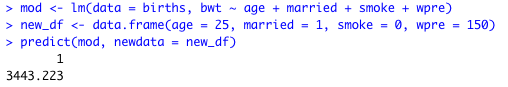
\includegraphics[scale=0.5]{newdata_example.png}
\end{figure}

\vspace{0.3cm}

\texttt{new\_df} is a dataframe containing a single row (one observation), for someone who is 25 years old, married, does not smoke, and weighed 150 pounds prior to pregnancy. It does all of the math for us!

\end{frame}

\begin{frame}{Prediction: Example in \texttt{R}}
We can also make predictions for multiple observations at the same time. For example, we can make predictions for all three of our examples from earlier using just a few lines of code:

\vspace{0.3cm}

\centering 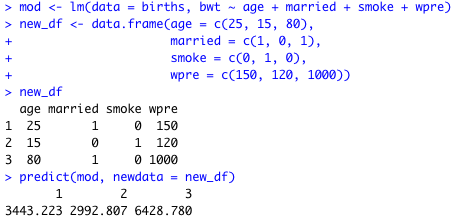
\includegraphics[scale=0.5]{newdata_example2.png}

\end{frame}

% could include a slide about thinking about which variables you can include in your model (i.e. not sex of child if we're predicting birthweight because not everyone knows the sex of their child before birth)

\section{Training and testing data}

\begin{frame}{Training and testing data}
Now that we are able to make predictions for new observations, we may be wondering how to tell whether or not we are predicting new observations \textit{well}. If our predictions are bad, they are not going to be particularly useful!

\vspace{0.3cm}

We care about ensuring that predictions are good for \textit{new observations}, rather than ensuring predictions are good for observations we have already observed. If we've already observed outcomes for certain individuals, we have no need to predict their outcomes (this would be redundant). Thus, we want to make sure our predictive model performs well on \textit{new} data, sometimes referred to as \textcolor{blue}{out-of-sample} data.

\vspace{0.3cm}

You may be wondering, how do we assess our model's performance on data that we have not yet collected?
\end{frame}

\begin{frame}
In practice, since we clearly do not have access to data that we have not yet collected, we instead pretend that some of the data we have in fact observed is ``new," and we try to accurately predict the observed outcomes on those ``new" observations. This involves splitting our dataset into \textcolor{blue}{training} and \textcolor{blue}{testing} data.

\vspace{0.3cm}

\textcolor{blue}{Training data:}

\vspace{0.3cm}

\textcolor{blue}{Testing data:}
\end{frame}

\section{Measures of prediction accuracy}

\subsection{$R^2$}
\subsection{Mean Squared Error}

\section{Bias-variance tradeoff}



\begin{frame}[c]
\centering \huge Any Questions?
\end{frame}

\end{document}